\chapter{Исследовательская часть}

\section{Технические характеристики}

Технические характеристики устройства, на котором выполнялись замеры по времени, представлены далее:

\begin{itemize}
	\item Процессор -- 2 ГЦ 4‑ядерный процессор Intel Core i5;
	\item Оперативная память -- 16 ГБайт;
	\item Операционная система -- macOS Venura 13.5.2. 
\end{itemize}

\section{Пример работы}

% \begin{figure}[h]
% 	\centering
% 	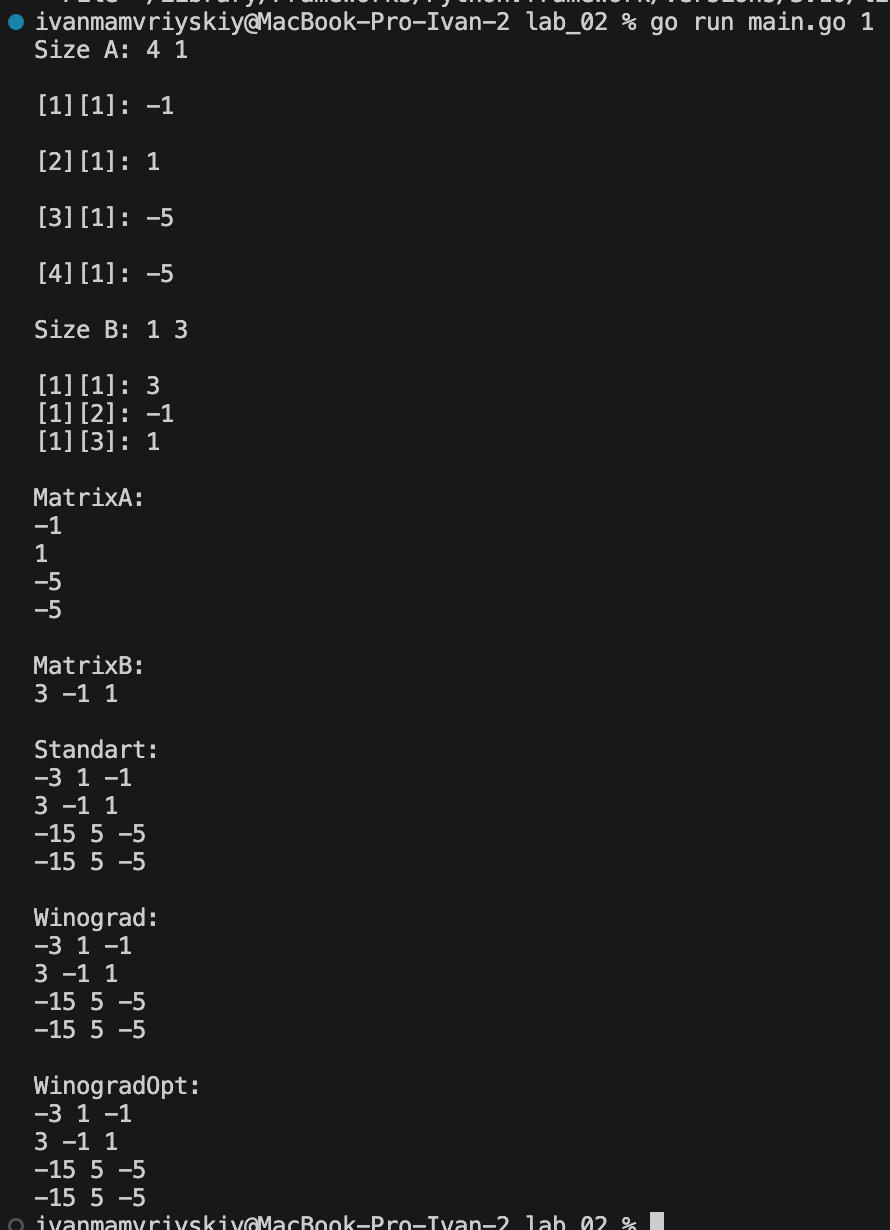
\includegraphics[height=0.4\textheight]{img/example.jpg}
% 	\caption{Демонстрация работы программы}
% 	\label{img:demonstration}
% \end{figure}

В данном подразделе представлен пример \ref{lst:exmpl} работы программы: 

\begin{lstlisting}[label=lst:exmpl,caption=Демонстрация работы алгоритма]
    ivanmamvriyskiy@MacBook-Pro-Ivan-2 main % go run main.go 1
    Size A: 4 1

    [1][1]: -1

    [2][1]: 1

    [3][1]: -5

    [4][1]: -5

    Size B: 1 3

    [1][1]: 3
    [1][2]: -1
    [1][3]: 1

    MatrixA:
    -1 
    1 
    -5 
    -5 

    MatrixB:
    3 -1 1 

    Standart:
    -3 1 -1 
    3 -1 1 
    -15 5 -5 
    -15 5 -5 

    Winograd:
    -3 1 -1 
    3 -1 1 
    -15 5 -5 
    -15 5 -5 

    WinogradOpt:
    -3 1 -1 
    3 -1 1 
    -15 5 -5 
    -15 5 -5 
\end{lstlisting}

\clearpage
\section{Время выполнения алгоритмов}

В таблице \ref{tab:time} представлены замеры времени для алгоримтов 
умножения матриц при четных размерностях. График зависимостей времени выполнения от размерности показан 
на графике \ref{img:dem}.
\begin{table}[!ht]
    \centering
    \caption{\label{tab:time}Замеры времени выполнения алгоритмов при четных размерностях(нс).}
    \begin{tabular}{|r|r|r|r|}
    \hline
        Размерность & Стандартный & Виноград & Виноград Оптимизир  \\ \hline
        10 & 4 & 6       &     5   \\ \hline
        100 & 4 131 &  2 506   & 2 169  \\ \hline
        200 & 20 429 &  18 960    & 19 138  \\ \hline
        300 & 72 264 & 64 371      &  63 638  \\ \hline
        400 & 195 449 & 189 089   &    178 892   \\ \hline
        500 & 503 049 & 387 605 &    329 304  \\ \hline
        600 & 684 740 & 680 307 &     665 368   \\ \hline
        700 & 1 455 149 & 1 773 952 &    1 269 319   \\ \hline
        800 & 1 615 890 & 1 418 696 &     1 517 012 \\ \hline
        900 & 3 383 536 & 3 272 015 &    2 740 418   \\ \hline
        1000 & 6 225 405 & 5 797 701 &   5 461 040  \\ \hline
    \end{tabular}
\end{table}

% \begin{figure}[h]
% 	\centering
% 	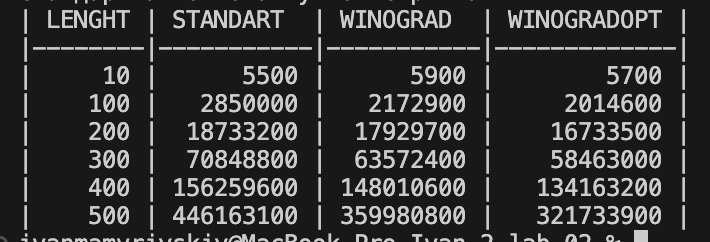
\includegraphics[height=0.15\textheight]{img/resTime.jpg}
% 	\caption{Результаты замера времени}
% 	\label{img:demonstration}
% \end{figure}

\begin{figure}[h]
	\centering
	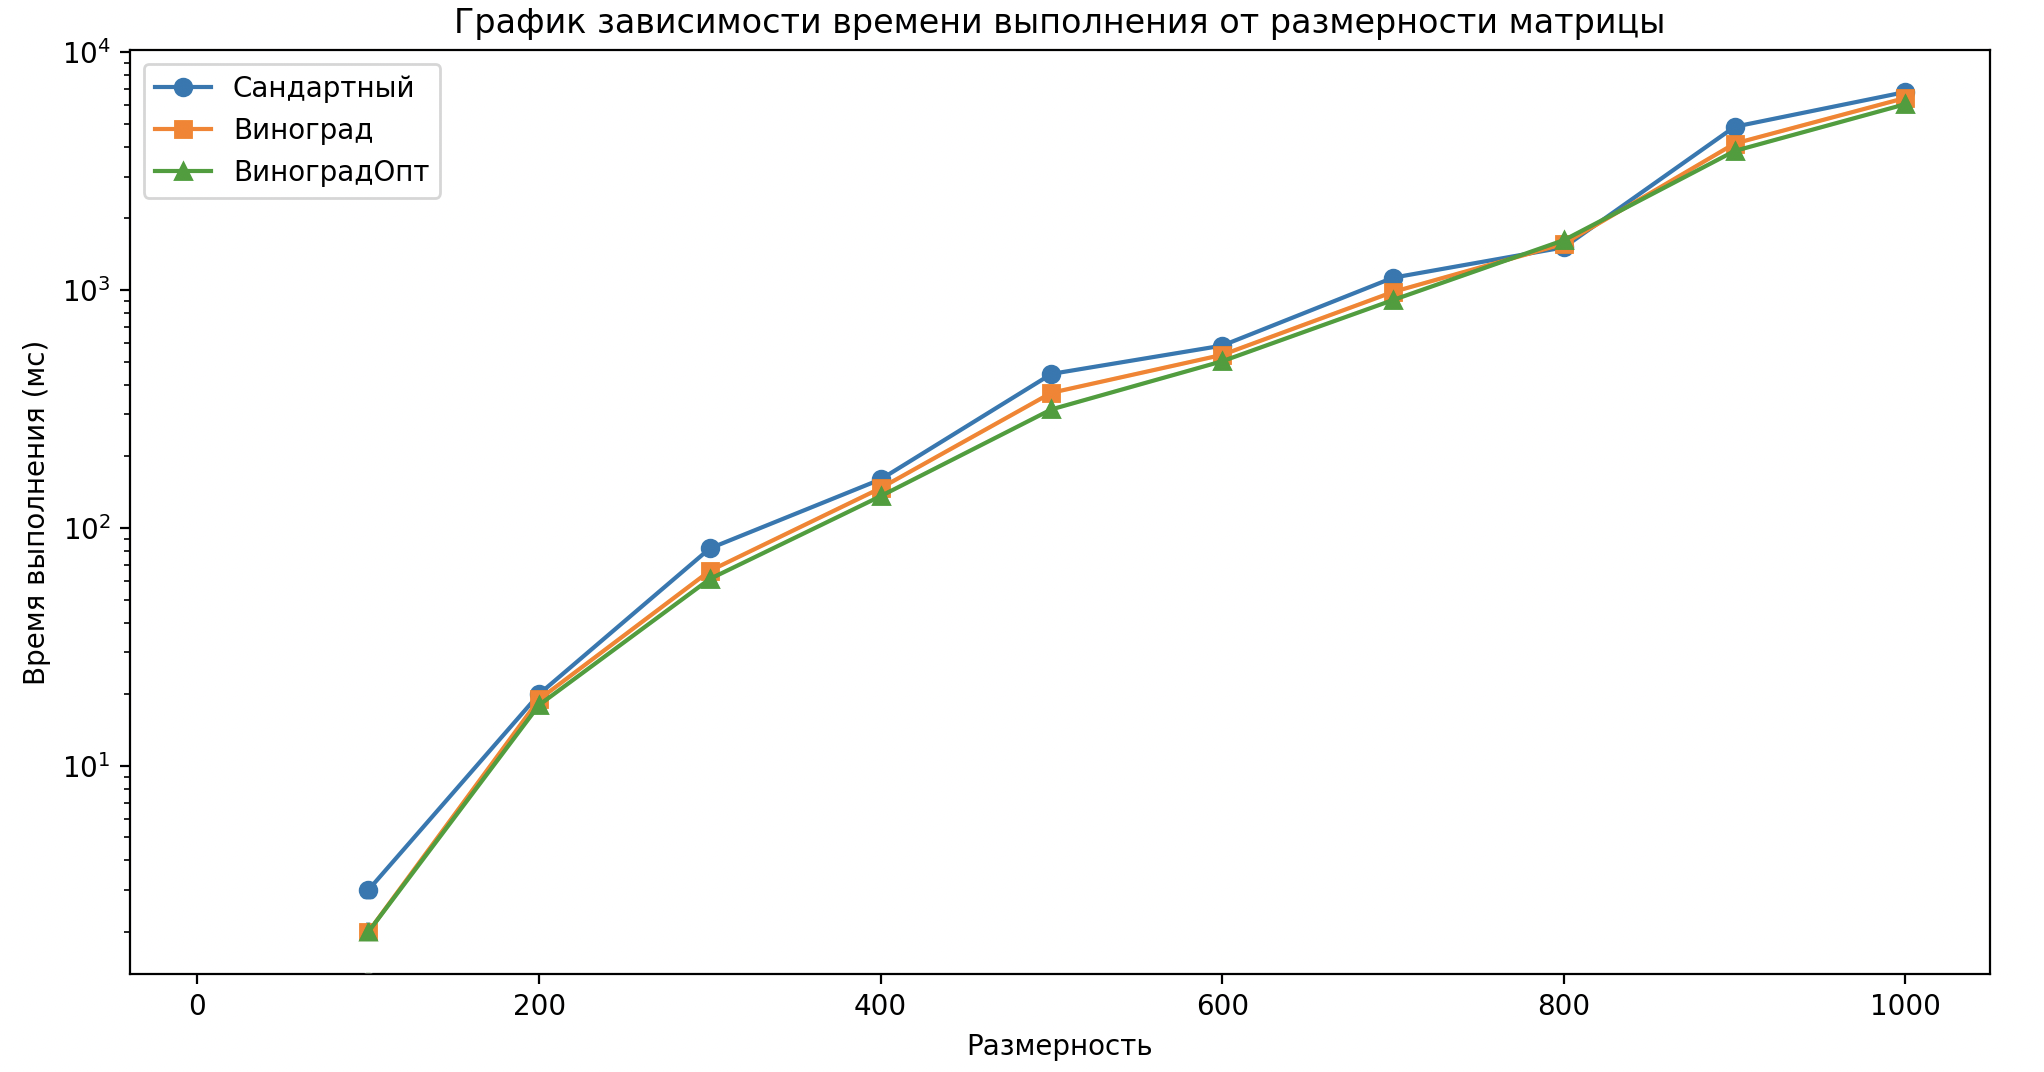
\includegraphics[height=0.35\textheight]{img/graph.png}
	\caption{График замера времени при четных размерностях}
	\label{img:dem}
\end{figure}

\clearpage

В таблице \ref{tab:time2} представлены замеры времени для алгоримтов 
умножения матриц при нечетных размерностях. График зависимостей времени выполнения от размерности показан 
на графике \ref{img:dem2}.

\begin{table}[!ht]
    \centering
    \caption{\label{tab:time2}Замеры времени выполнения алгоритмов при нечетных размерностях(нс).}
    \begin{tabular}{|r|r|r|r|r|}
    \hline
        Размерность & Стандартный & Виноград & Виноград Оптимизир   \\ \hline
        11 & 6 & 7 & 6   \\ \hline
        101 & 2 819 & 2 525 & 2 407   \\ \hline
        201 & 20 040 & 18 278 & 17 336   \\ \hline
        301 & 69 682 & 62 652 & 57 036   \\ \hline
        401 & 158 474 & 146 123 & 135 236   \\ \hline
        501 & 439 145 & 356 716 & 313 788   \\ \hline
        601 & 575 588 & 527 767 & 494 750   \\ \hline
        701 & 1 128 277 & 959 669 & 898 226   \\ \hline
        801 & 1 473 640 & 1 381 828 & 1 279 278   \\ \hline
        901 & 4 678 927 & 4 444 102 & 4 153 936   \\ \hline
        1001 & 7 007 630 & 6 864 435 & 6 789 342  \\ \hline
    \end{tabular}
\end{table}

\begin{figure}[h]
	\centering
	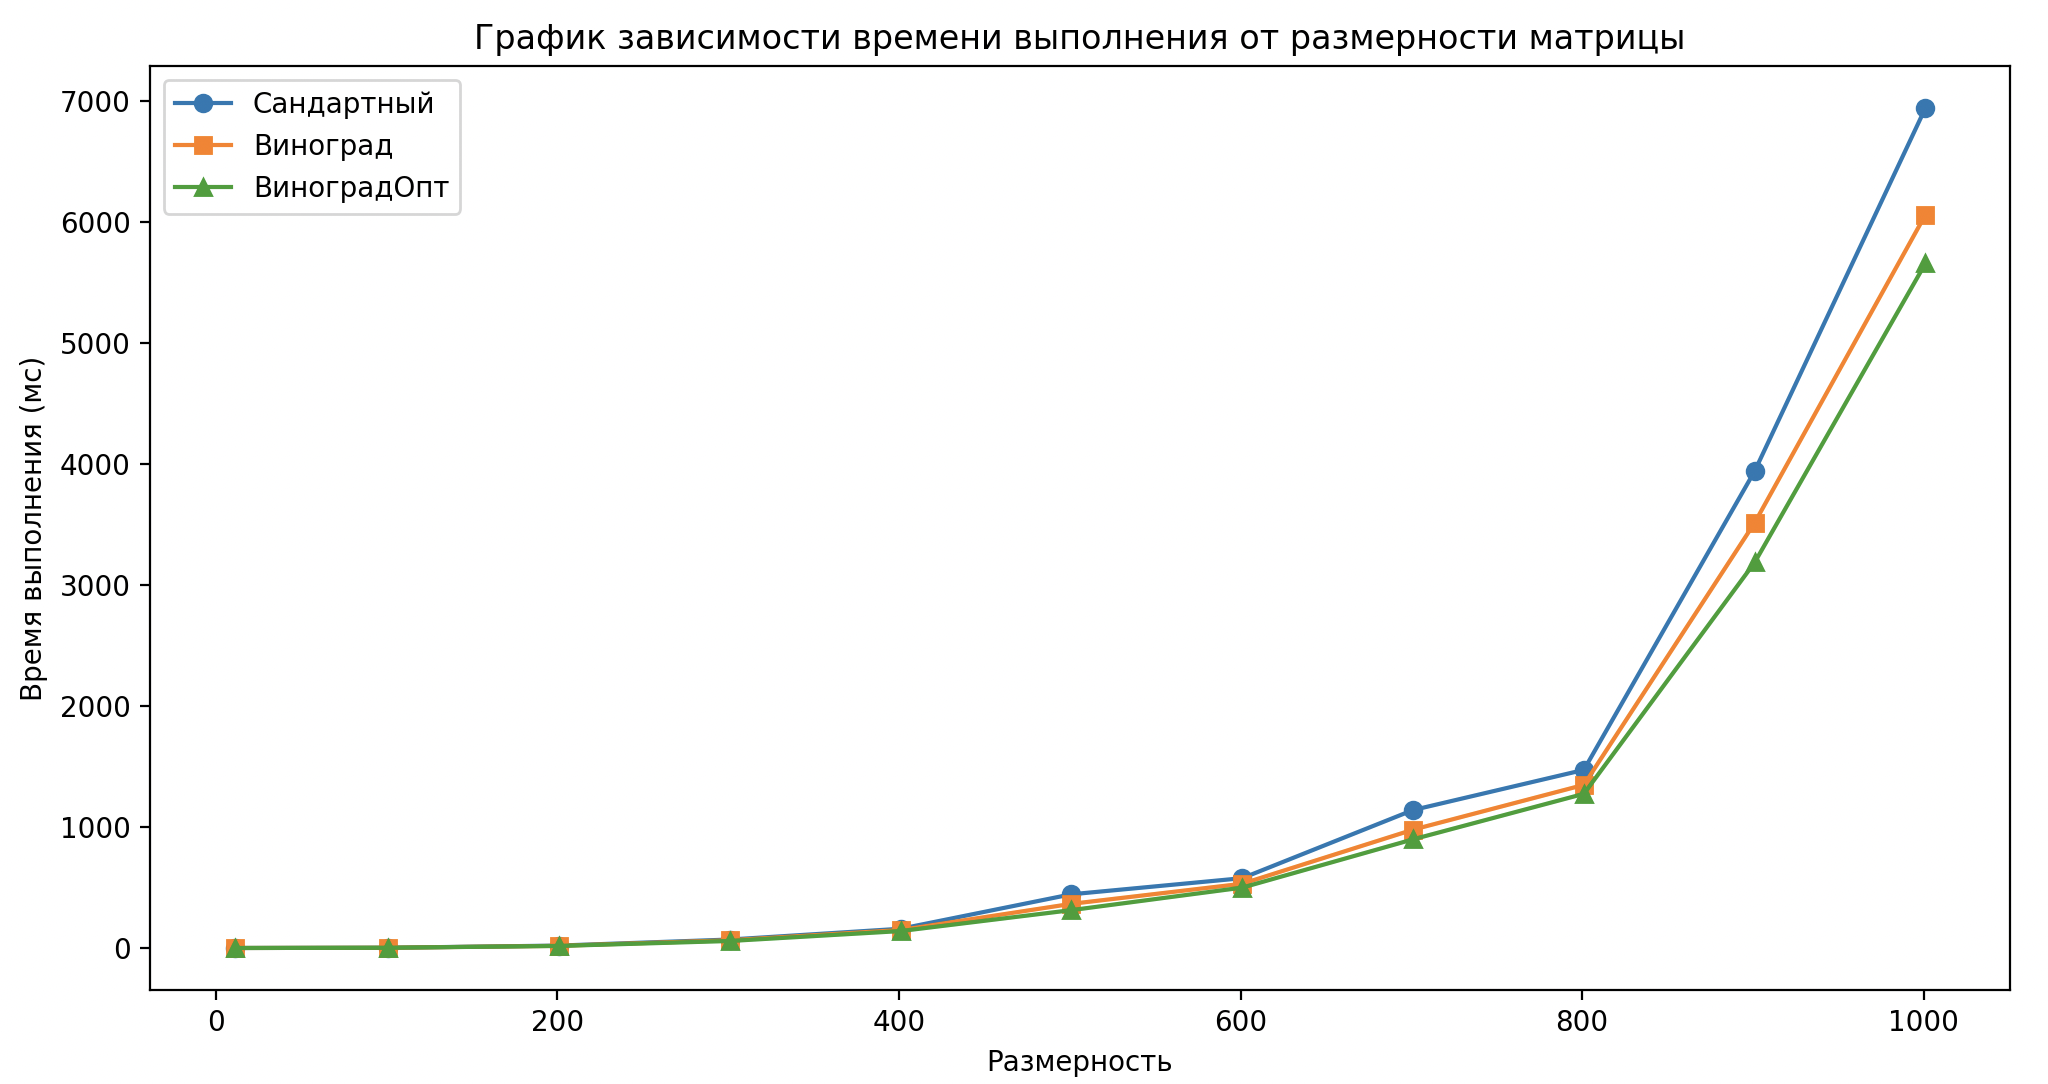
\includegraphics[height=0.35\textheight]{img/graph123.png}
	\caption{График замера времени при нечетных размерностях}
	\label{img:dem2}
\end{figure}


\clearpage

\section{Замеры памяти при выполнении алгоритмов}

В таблице \ref{tab:table} представлены результаты замера памяти алгоритмов умножения
матриц при четной размерности, в таблице \ref{tab:tabl} при нечетной размерности.

\begin{table}[!ht]
    \centering
    \caption{\label{tab:table}Замеры памяти при выполнении алгоритмов для четных размерностец матриц}
    \begin{tabular}{|r|r|r|r|r|r|}
    \hline
        Длина & Стандартный & Виноград & Виноград Опт   \\ \hline
        10 & 1 040 & 1 200 & 1 200   \\ \hline
        100 & 92 288 & 94 080 & 94 080   \\ \hline
        200 & 363 264 & 366 848 & 366 848   \\ \hline
        300 & 814 592 & 819 968 & 819 968   \\ \hline
        400 & 1 289 728 & 1 296 128 & 1 296 128   \\ \hline
        500 & 2 060 288 & 2 068 480 & 2 068 576   \\ \hline
        600 & 2 937 032 & 2 944 512 & 2 944 512   \\ \hline
        700 & 4 319 232 & 4 331 616 & 4 331 520   \\ \hline
        800 & 5 242 880 & 5 255 936 & 5 255 936   \\ \hline
        900 & 7 394 560 & 7 411 040 & 7 410 944   \\ \hline
        1000 & 8 216 576 & 8 232 960 & 8 232 960  \\ \hline
    \end{tabular}
\end{table}

\begin{table}[!ht]
    \centering
    \caption{\label{tab:tabl}Замеры памяти при выполнении алгоритмов для нечетных размерностец матриц(байт).}
    \begin{tabular}{|r|r|r|r|r|r|}
    \hline
    Длина & Стандартный & Виноград & Виноград Опт   \\ \hline
        11 & 1 344 & 1 536 & 1 536   \\ \hline
        101 & 93 184 & 94 976 & 94 976   \\ \hline
        201 & 365 056 & 368 640 & 368 640   \\ \hline
        301 & 817 288 & 822 656 & 822 664   \\ \hline
        401 & 1 395 584 & 1 402 496 & 1 402 496   \\ \hline
        501 & 2 064 384 & 2 072 576 & 2 072 576   \\ \hline
        601 & 2 939 648 & 2 949 376 & 2 949 376   \\ \hline
        701 & 4 325 376 & 4 337 664 & 4 337 664   \\ \hline
        801 & 5 249 408 & 5 262 464 & 5 262 464   \\ \hline
        901 & 7 402 752 & 7 419 136 & 7 419 136   \\ \hline
        1001 & 8 224 768 & 8 241 152 & 8 241 152  \\ \hline
    \end{tabular}
\end{table}

\clearpage
\section{Вывод}

По результатам эксперимента можно сделать следующие выводы:
\begin{itemize}[left=\parindent]
    \item прямая реализация алгоритма Винограда без какой-либо опитимизации
        работает примерно в 1.2 раза быстрее стандартного алгоритма;
    \item оптимизированная версия Винограда работает в 1.4 раза быстрее
        стандартного алгоритма;
    \item при нечетных размерностях алгоритм Винограда работает дольше, чем при четных размерностях;
    \item алгоритм Винограда тратит больше памяти, чем стандартный алгоритм, так как
        происходит предварительная обработка.
\end{itemize}

Таким образом, для вычисления произведения матриц при необходимости меньшего времени вычисления
следует использовать оптимизированный алгоритм Винограда.
